%\documentclass[12pt,a4paper,dvipsnames,usenames]{beamer}
\documentclass[12pt,a4paper,dvipsnames,usenames,handout]{beamer}
\usepackage{url}
\usepackage{xcolor}
\usepackage{amsmath,varwidth,slashed}
\usepackage[utf8]{inputenc}
\usepackage[T1]{fontenc}
\usepackage{tikz,xparse}
\usepackage[normalem]{ulem}
\usepackage{transparent}
\usepackage{appendixnumberbeamer}

% -------------------------- %
% Standard LaTeX definitions %
% -------------------------- %

\DeclareGraphicsExtensions{.pdf}
\renewcommand\textbullet{\ensuremath{\bullet}}

% ----------------------------------- %
% Various tikz styles and definitions %
% ----------------------------------- %

\usetikzlibrary{calc,intersections,positioning,matrix,chains,scopes}
\usetikzlibrary{decorations.pathmorphing,decorations.pathreplacing,shapes}
\newcommand{\tikzmark}[1]{\tikz[overlay,remember picture] \node (#1) {};}

\tikzumlset{fill class=RoyalBlue!20}

\tikzstyle{startnode} = [circle, draw, fill=Bittersweet!20, minimum size=10pt, inner sep = 0]
\tikzstyle{stopnode} = [startnode]
\tikzstyle{process} = [rectangle, minimum width=2cm, minimum height=.7cm, text centered, draw, fill=OliveGreen!20, align=center, font=\scriptsize]
\tikzstyle{dangerprocess} = [process, fill=BrickRed!20, draw=BrickRed, thick]
\tikzstyle{flowarrow} = [->, >=stealth, thick]

% ---------------------------------- %
% My default listings C++ code style %
% ---------------------------------- %

\lstset{%
  language=C++, basicstyle=\scriptsize\ttfamily, 
  keywordstyle=\color{OliveGreen}, identifierstyle=\color{RoyalBlue}, 
  commentstyle=\color{Brown}, stringstyle=\color{Bittersweet}, showstringspaces=false,  
  breaklines=true, prebreak=\mbox{{\color{Bittersweet}\tiny\ $\hookleftarrow$}}, 
  postbreak=\mbox{{\color{Bittersweet}\tiny$\to$\ }}, tabsize=5,
  morekeywords={%
    MyClass,unique_ptr,shared_ptr,weak_ptr,auto_ptr,
    make_unique, make_shared, default_delete,
    dynamic_pointer_cast, const_pointer_cast,
    scoped_ptr,QSharedPointer,QScopedPointer,QWeakPointer,
    ftring, SmartPtr, Shape, Circle, ShapeFactory, CircleFactory,
    Derived, Base
  }
}

\def\inline{\lstinline[basicstyle=\ttfamily\normalsize]}

% ---------------------------------------------------------------------------------------------------- %
% Various command for inline code instead of lstinline so that I don't have to update the keyword list %
% ---------------------------------------------------------------------------------------------------- %

\newcommand{\object}[1]{{\ttfamily \color{OliveGreen}#1}}
\newcommand{\function}[1]{{\ttfamily \color{RoyalBlue}#1}}
\newcommand{\std}[1]{{\ttfamily {\color{RoyalBlue} std::}{\color{OliveGreen}#1}}}
\newcommand{\boost}[1]{{\ttfamily {\color{RoyalBlue} boost::}{\color{OliveGreen}#1}}}

\newcommand{\uniqueptr}{\std{unique\_ptr}}
\newcommand{\sharedptr}{\std{shared\_ptr}}
\newcommand{\weakptr}{\std{weak\_ptr}}
\newcommand{\autoptr}{\std{auto\_ptr}}

% The base16 colour scheme?
\definecolor{sbase03}{HTML}{002B36}
\definecolor{sbase02}{HTML}{073642}
\definecolor{sbase01}{HTML}{586E75}
\definecolor{sbase00}{HTML}{657B83}
\definecolor{sbase0}{HTML}{839496}
\definecolor{sbase1}{HTML}{93A1A1}
\definecolor{sbase2}{HTML}{EEE8D5}
\definecolor{sbase3}{HTML}{FDF6E3}
\definecolor{syellow}{HTML}{B58900}
\definecolor{sorange}{HTML}{CB4B16}
\definecolor{sred}{HTML}{DC322F}
\definecolor{smagenta}{HTML}{D33682}
\definecolor{sviolet}{HTML}{6C71C4}
\definecolor{sblue}{HTML}{268BD2}
\definecolor{scyan}{HTML}{2AA198}
\definecolor{sgreen}{HTML}{859900}

\definecolor{Tropiteal}{RGB}{0,168,198}
\definecolor{TealDrop}{RGB}{64,192,203}
\definecolor{WhiteTrash}{RGB}{249,242,231}
\definecolor{AtomicBikini}{RGB}{174,226,57}
\definecolor{FeebleWeek}{RGB}{143,190,0}
\definecolor{ICantExpress}{RGB}{28,20,13}
\definecolor{Marty}{RGB}{250,42,0}

\colorlet{ColourBase}{Tropiteal}
\colorlet{ColourHl1}{Marty}
\colorlet{ColourHl2}{FeebleWeek}
\colorlet{ColourHl3}{TealDrop}
\colorlet{ColourDark}{ICantExpress}
\colorlet{ColourDark2}{Tropiteal}


\usetheme{metropolis}

\setbeamercolor{alerted text}{%
  fg=bazelGreen
}

\setbeamercolor{example text}{%
  fg=mLightBrown
}

\setbeamercolor{frametitle}{%
  use=normal text,
  fg=normal text.bg,
  bg=bazelGreen
}

\lstset{%
  basicstyle=\ttfamily\lst@ifdisplaystyle\fontsize{9pt}{9pt}\selectfont\fi,
  keywordstyle=\color{sgreen}, identifierstyle=\color{sblue}, 
  commentstyle=\color{sbase1}, stringstyle=\color{sorange},
  numberstyle=\color{sviolet}, showstringspaces=false,  
  breaklines=true,
  tabsize=5,
}

\lstalias[]{gnumake}[gnu]{make}

\newcommand{\dimtext}[2]%
{
  { \transparent{0.7}
  \begin{tikzpicture}[overlay, remember picture]
    \fill[white] ( #1 -| current page.north west) -- ++(0,.8em) -- ++(\paperwidth,0) -- (#2 -| current page.north east)
   -- ++(0,-.5em) -- ++(-\paperwidth,0) -- cycle;
  \end{tikzpicture}
  }
}

\newcommand{\specialcell}[2][c]{%
  \begin{tabular}
    [#1]{@{}c@{}}#2
  \end{tabular}
}

\newcommand{\tikzmark}[1]{\tikz[overlay,remember picture] \coordinate (#1);}

\newcommand{\qmat}{\ensuremath{Q_{\mathrm{uark}}}}
\newcommand{\mathfont}{\fontsize{10pt}{12pt}}
\newcommand{\minus}{\scalebox{0.75}[1.0]{$-$}}
\newcommand{\sectionframe}{%
  \addtocounter{framenumber}{-1}%
  \frame[plain]{\begin{center}\LARGE \color{beameralert} \insertsection\end{center}}}

\newcommand{\breakline}{%
  \begin{center} \begin{tikzpicture}
      \draw[beamerprimary] ({-0.5 * \textwidth},0) -- ({0.5 * \textwidth},0);
      \node[inner sep=0, minimum size=7pt, fill=white,circle] {};
      \node[inner sep=0, minimum size=4pt, draw=beamerprimary,circle] {};
      \node[inner sep=0, minimum size=1pt, fill=beamerprimary,circle] {};
  \end{tikzpicture} \end{center}
}


\setbeameroption{show notes}

%\title{\strut{}Analytic computations \strut{}of an effective lattice \strut{}theory for heavy quarks}
\title{Analytic computations of an effective lattice theory for heavy quarks}
\author{\underline{Aleksandra R. Glesaaen}\\[2pt]\small Mathias Neuman, Owe Philipsen}% \\ \texttt{glesaaen@th.physik.uni-frankfurt.de}}
\institute{
\includegraphics[scale=0.08]{Figs/GU-Logo-blau-CMYK.pdf}}
\date{Lattice Conference 2015 - July 16th}

\begin{document}

\setlength{\abovedisplayskip}{0pt}
\setlength{\belowdisplayskip}{0pt}

\begin{frame}[plain]
  \titlepage
\end{frame}

\setcounter{framenumber}{0}

\begin{frame}[plain]
  \tableofcontents
\end{frame}

\begin{frame}
  \frametitle{Heavy QCD Phase Diagram}

  {\centering
    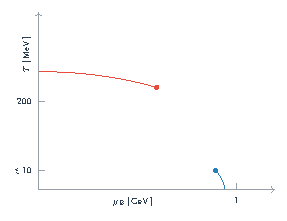
\includegraphics[width=\textwidth]{Figs/heavy_qcd_phase_diag_no_title.pdf}
  \par}

  \uncover<2>{
  \begin{tikzpicture}[overlay,remember picture]
    \draw[<-,>=stealth] ([shift={(-3.4,1.8)}] current page.south east) .. controls +(.7,.7) and +(0,-1) .. +(0.5,2)
      node[above=.2,scale=0.75,align=center] {Liquid Gas\\Phase Transition};
  \end{tikzpicture}
  }

\end{frame}

\begin{frame}
  \frametitle{Advantages of the Effective Theory}

  \begin{itemize}
    \setlength\itemsep{2em}
    \item Dimensionally reduced theory
    \begin{itemize}
      \item $4$D $\to 3$D
      \item $U_{\mu}(x) \to L(x)$
    \end{itemize}
    \item Very mild sign problem, most gauge fields integrated analytically
    \item Want to study the very dense limit, liquid gas transition
  \end{itemize}

\end{frame}

\section{The Effective Theory}

\sectionframe

\begin{frame}
  \frametitle{The Effective Lattice Theory}

  \begin{alertblock}{Effective Theory}
    \begin{itemize}
      \item \color{LightUIBase} Integrate out all spatial gauge links
    \end{itemize}
    \begin{align*}
      \mathcal{Z} &= \int D U_{\mu} \exp\big\{ \minus S_{\mathrm{action}} \big\} \\
      &= \int D U_0 \exp\big\{ \minus S_{\mathrm{effective \: action}} \big\}
    \end{align*}
  \end{alertblock}

  \vspace{1em}

  {\color{LightUIRed}Using:}
  \begin{itemize}
    \item The strong coupling expansion
    \item The hopping parameter expansion
  \end{itemize}

\end{frame}

\begin{frame}
  \frametitle{}

  \begin{block}{Effective Theory}
    \begin{equation} \tag{$\dagger$} \label{eq:eff}
      \mathcal{Z} = \int \prod_x \mathrm{d} L(x) \, \exp \big\{ \minus S_{\mathrm{eff \: action}} \big\}
    \end{equation}
  \end{block}

  \vspace{1em}

  \begin{itemize} \setlength\itemsep{2em}
    \item Previous Talk: Monte Carlo simulations of \eqref{eq:eff}
    \item Current Talk: Analytic calculation of $\mathcal{Z}$
  \end{itemize}

\end{frame}

\begin{frame}
  \frametitle{The Effective Theory Action}

  \only<1-2|handout:1>{
  \begin{block}{}
    \[
      S_{\mathrm{eff \: action}} = S_0\big[L\big] + S_I\big[L\big]
    \]
  \end{block}

  \vspace{1em}

  Where $S_I\big[L\big]$ is made up of interactions at varying distances
  }

  
  \vspace{1em}

  \begin{block}{}
    \[
      S_I\big[ L \big] = \sum_{\vphantom{d}\mathrm{terms}} \sum_{\mathrm{dof}} v_i(1,2,...,n_i) \phi_1 \big[L\big] \phi_2 \big[L\big] \cdots
      \phi_{n_i} \big[ L \big]
    \]
  \end{block}
  
  \vspace{1em}

  \only<3|handout:2>{
    {\color{LightUIRed} In our theory:}
    \vspace{1ex}
    \begin{itemize}
      \setlength\itemsep{1em}
      \item $v_i(1,2,...n_i) \to \big\{ \lambda_i, h_i \big\} \times \mathrm{geometry}$
      \item $\phi_i \to \big\{ L_i, L_i^*, W_i \big\}$
    \end{itemize}
  }

  \only<1-2|handout:1>{
  \begin{tikzpicture}[overlay,remember picture]
    \only<2>{
    \coordinate (vcoord) at ([shift={(-1.5,2.5)}] current page.south);
    \draw[<-,>=stealth] (vcoord) .. controls +(0,-2.5) and +(-.5,0) .. +(2,-1.5)
      node[right,align=left,scale=0.85] {Can be represented\\with connected graphs};
    }
  \end{tikzpicture}
  }

  \note<1-2|handout:1>
  {
    Remember to say that the effective couplings $V_i$ are themselves functions of $\kappa$ and $\beta$, and we can therefore
    carry out a consistent expansion.

    Talk about the expansion point. What is $S_0$ physically? Free hadron gas.
  }
\end{frame}

\begin{frame}
  \frametitle{Analytic Calculations}
  \framesubtitle{N-point Linked Cluster Expansion}

  {\color{LightUIBlue}\large Classical Linked Cluster Expansion} \\[5pt]
  The action consists of two-point interactions which can be expanded in a set of connected graphs.

  \vspace{2em}

  {\color{LightUIBlue}\large Our Problem} \\[5pt]
  The action contains $n$-point interactions that we can embed on a set of connected graphs. \\[5pt]
  \hspace{1em}\tikz[baseline={-3pt},rounded corners=2pt] \draw[->,>=stealth] (0,.2) -- (0,0) -- (.5,0);
  Two step embedding

\end{frame}

\begin{frame}
  \frametitle{Analytic Calculations}
  \framesubtitle{N-point Linked Cluster Expansion}

  {\centering
    \begin{tikzpicture}
      \node[scale=0.75] (title1) {\strut{}Effective Action Term};
      \node[below=2pt of title1] (graphs1) {
\includegraphics{Graphs/graph1.pdf} \hspace{1em} 
\includegraphics{Graphs/graph2.pdf}};
      \node (fit1) [draw=LightUIBlue,rounded corners=2pt] [fit={(title1) (graphs1)}] {};

      \node[right=1.5cm of title1] (title2) [scale=0.75] {Skeleton Graph};
      \node[below=2pt of title2] (graphs2) [inner ysep=7.5pt] {\includegraphics{Graphs/graph_skel.pdf}};
      \node (fit2) [draw=LightUIBlue,rounded corners=2pt] [fit={(title2) (graphs2)}] {};

      \node (e1) at ([shift={(-2.2cm,-3cm)}] fit1.south) {\includegraphics{Graphs/graph_emb3.pdf}};
      \node[right=of e1] (e2) {\includegraphics{Graphs/graph_emb1.pdf}};
      \node[right=of e2] (e3) {\includegraphics{Graphs/graph_emb2.pdf}};
      \node[right=of e3] (e4) {\includegraphics{Graphs/graph_emb4.pdf}};

      \node (fit3) [draw=LightUIBlue,rounded corners=2pt] [fit={(e1) (e2) (e3) (e4)}] {};

      \coordinate (merge) at ([yshift=1.6cm] fit3.north);

      \draw[LightUIBlue,rounded corners=3pt] (fit1.south) |- (merge) -- (fit3.north);
      \draw[->,>=stealth,LightUIBlue,rounded corners=3pt] (fit2.south) |- (merge) -- (fit3.north)
        node[scale=0.75,text=LightUIBase,midway,right] {embedding};

    \end{tikzpicture}
  \par}

\end{frame}

\begin{frame}[plain]
  \begin{tikzpicture}[overlay,remember picture]
    \node[anchor=north] at ([shift={(0,.3)}] current page.north)
    {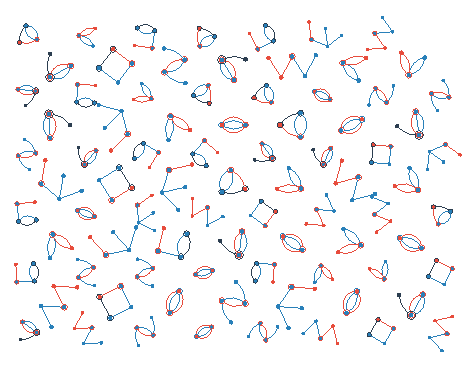
\includegraphics[scale=1.6]{Graphs/graphmatrix.pdf}};
  \end{tikzpicture}
\end{frame}

\begin{frame}
  \frametitle{The power of resummations}
  
  Using the resummed Linked Cluster Expansion as motivation

  \vspace{2em}

  {\centering
    \includegraphics[scale=0.9]{Graphs/graph_renorm.pdf}
  \par}

  \vspace{2em}

  We can do the same resummation for the effective action itself, incorporating long-range effects

\end{frame}

\section{Results}

\sectionframe

\begin{frame}
  \frametitle{Convergence}

  {\centering%
    \only<1|handout:0>{\includegraphics[width=\textwidth]{Plots/resummed_conv_part1.pdf}}%
    \only<2|handout:0>{\includegraphics[width=\textwidth]{Plots/nucleon_compare_part1.pdf}}%
    \only<3|handout:1>{\includegraphics[width=\textwidth]{Plots/nucleon_compare_part2.pdf}}%
  \par}

  \begin{tikzpicture}[overlay,remember picture]
    \draw[->,>=stealth] ([shift={(2.5,1.15)}] current page.south) -- +(2,0)
      node[midway,below,scale=0.65] {$m_q \to 0$};
    \node[anchor=west] at ([shift={(-.7,-2.3)}] current page.north) [scale=0.8] {$h_1 = \kappa^{N_t} e^{N_t \mu} = 0.8$};
  \end{tikzpicture}

  \note
  {
    Say something about the fact that higher $h_2$ means smaller quark masses.
  }
\end{frame}

\begin{frame}
  \frametitle{Effect of the resummations}

  {\centering%
    \only<1|handout:0>{\includegraphics[width=\textwidth]{Plots/resummed_conv_part2.pdf}}%
    \only<2|handout:1>{\includegraphics[width=\textwidth]{Plots/resummed_conv_part3.pdf}}%
  \par}

  \begin{tikzpicture}[overlay,remember picture]
    \draw[->,>=stealth] ([shift={(2.5,1.15)}] current page.south) -- +(2,0)
      node[midway,below,scale=0.65] {$m_q \to 0$};
    \node[anchor=west] at ([shift={(-.7,-2.3)}] current page.north) [scale=0.8] {$h_1 = \kappa^{N_t} e^{N_t \mu} = 0.8$};
  \end{tikzpicture}
\end{frame}

\begin{frame}
  \frametitle{Effect of the resummations}

  {\centering%
    \only<1|handout:0>{\includegraphics[width=\textwidth]{Plots/resummed_conv_part4.pdf}}%
    \only<2|handout:0>{\includegraphics[width=\textwidth]{Plots/resummed_conv_part5.pdf}}%
    \only<3|handout:1>{\includegraphics[width=\textwidth]{Plots/resummed_conv_part6.pdf}}%
  \par}

  \begin{tikzpicture}[overlay,remember picture]
    \draw[->,>=stealth] ([shift={(2.5,1.15)}] current page.south) -- +(2,0)
      node[midway,below,scale=0.65] {$m_q \to 0$};
    \node[anchor=west] at ([shift={(-.7,-2.3)}] current page.north) [scale=0.8] {$h_1 = \kappa^{N_t} e^{N_t \mu} = 1.0$};
  \end{tikzpicture}
\end{frame}

\begin{frame}
  \frametitle{Binding energy}

  {\centering
    \includegraphics[width=\textwidth]{Plots/binding_energy.pdf}
  \par}

  \begin{tikzpicture}[overlay,remember picture]
    \node[text=LightUIBase,scale=0.75] at ([shift={(1,-2)}] current page.north) [anchor=west] {$\epsilon = \displaystyle\frac{e - m_B n_B}{m_B n_B}$};
  \end{tikzpicture}

  \note
  {
    Plot parameters: $\kappa = 0.08, N_t = 50, \beta = 0$
  }

\end{frame}

\begin{frame}
  \frametitle{Continuum comparison}

  {\centering
    \includegraphics[width=\textwidth]{Plots/nbVmu_comp.pdf}
  \par}

\end{frame}

\begin{frame}
  \frametitle{Continuum Equation of State}

  {\centering
    \includegraphics[width=\textwidth]{Plots/nbVpress_c2000.pdf}
  \par}

\end{frame}

\section{Conclusion}

\sectionframe

\begin{frame}
  \frametitle{Summary \& Outlook}

  \only<1|handout:1>{
  {\color{LightUIRed} Summary}
  \begin{itemize}
    \setlength\itemsep{1em}
    \item Introduced the effective dimensionally reduced lattice theory
    \item Looked at how a consistent analytic calculation could be carried out
    \item Demonstrated convergence and comparisons with numerics
  \end{itemize}
  }

  \only<2|handout:2>{
  {\color{LightUIRed} Outlook}
  \begin{itemize}
    \setlength\itemsep{1em}
    \item Use the analytic results as a tool to study the characteristics of the effective theory
    \item Find analytic resummation schemes to incorporate long-range effects
  \end{itemize}
  }
\end{frame}

\addtocounter{framenumber}{-1}
\frame[plain]{\begin{center}\LARGE \color{beameralert} Thank you!\end{center}}


\appendix
\section{Backup slides}
\sectionframe

\begin{frame}
  \frametitle{The Effective Lattice Theory}
  \framesubtitle{Pure gluon contributions}

  \only<1-3|handout:1>{
  \begin{center}
    \only<1|handout:0>{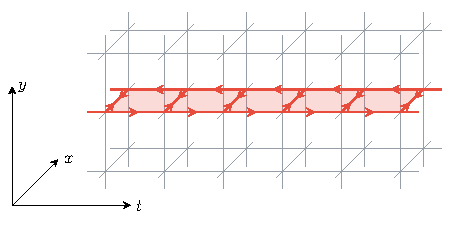
\includegraphics{Figs/puregauge1.pdf}}
    \only<2|handout:0>{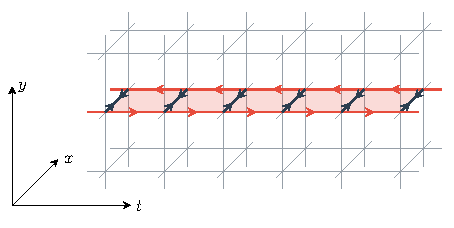
\includegraphics{Figs/puregauge2.pdf}}
    \only<3|handout:1>{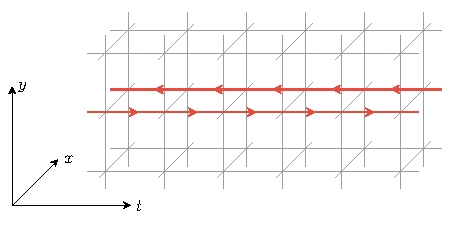
\includegraphics{Figs/puregauge3.pdf}}
  \end{center}
  }


  \only<1|handout:0>{
    Put a line of plaquettes in the time direction
  }
  \only<2|handout:0>{
    Integrate over all spatial gauge links
  }
  \only<3|handout:1>{
  What remains is an interaction between Polyakov Loops
  }

  \begin{onlyenv}<4|handout:2>

    \begin{block}{Effective Gluon Interactions}
      \begin{equation*}
        S_{\mathrm{eff \: gluon}} \sim \lambda \sum_{\langle x,y \rangle} L(x) L^*(y)
      \end{equation*}
    \end{block}

    \vspace{1em}

    \begin{center}
    \begin{tikzpicture}
      \draw[LightUIBase!50!white,use as bounding box] (-.3,-.3) grid[xstep=2] (6.3,2.3);
      \draw[thick,decorate, decoration={snake}, draw=LightUIBase] (2,1) -- (4,1)
        node[scale=0.75,midway,below=.2] {$\lambda$};
      \node[scale=2,fermion,fill=LightUIRed] at (4,1) (ell) {};
      \node[scale=0.75,above right=3pt of ell] {$L$};
      \node[scale=2,draw=LightUIRed, thick, circle, inner sep=0pt, minimum size=4pt] at (2,1) (elles) {};
      \node[scale=0.75,above left=3pt of elles] {$L^*$};

      \coordinate (coordcenter) at (-1,-1);
      \draw[->,>=stealth] (coordcenter) -- +(2,0) node[right,scale=0.75] {$x$};
      \draw[->,>=stealth] (coordcenter) -- +(0,2) node[right,scale=0.75] {$y$};
    \end{tikzpicture}
    \end{center}
     
    \vspace{1em}
  \end{onlyenv}

  \onslide<3|handout:1>{
  \begin{tikzpicture}[overlay, remember picture]
    \draw[<-,>=stealth] ([shift={(2.5,-.05)}] current page.center) .. controls +(.1,-.7) and +(-.3,0) .. +(2,-.4)
      node[scale=0.75,right] {$L$};
    \draw[<-,>=stealth] ([shift={(2.7,.5)}] current page.center) .. controls +(.1,.7) and +(-.3,0) .. +(2,+.4)
      node[scale=0.75,right] {$L^*$};
  \end{tikzpicture}
  }

  \note<3>
  {
    As mentioned earlier, we are only interested in quantities that contribute to the thermodynamic of the system. For our system,
    that means quantities which span the full temporal direction, and thus picks up a temperature dependent component in the
    infinite volume limit.

    For pure gauge action, in the strong coupling expansion, this means a plane of plaquettes spanning the full temporal
    direction, as shown in the figure. We then integrate out the spatial links present in this strip of plaquettes, and are left
    with the Polyakov loops.
  }

  \note<4>
  {
    The final result will thus be a nearest neighbour interaction between two Polyakov loops, or a continuos spin-system on a
    three dimensional lattice.
  }
\end{frame}

\begin{frame}
  \frametitle{The Effective Lattice Theory}
  \framesubtitle{Pure quark contributions}

  \only<1-3|handout:1>{
  \begin{center}
    \only<1|handout:0>{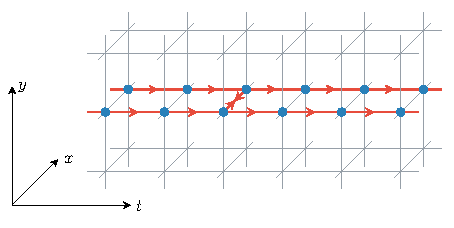
\includegraphics{Figs/purequark1.pdf}}
    \only<2|handout:0>{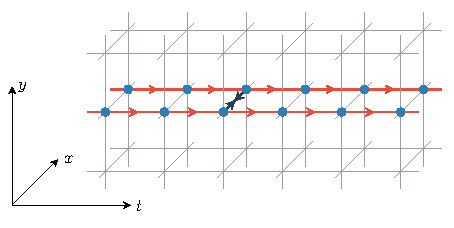
\includegraphics{Figs/purequark2.pdf}}
    \only<3|handout:1>{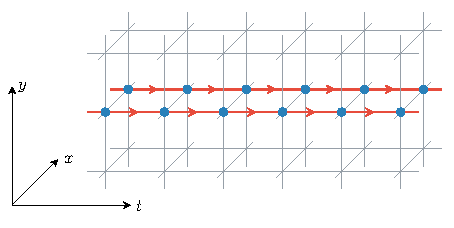
\includegraphics{Figs/purequark3.pdf}}
  \end{center}
  }

  \only<1-3|handout:1>{
  \begin{overlayarea}{\textwidth}{3em}
  \only<1|handout:0>{
    Can produce a closed quark loop with multiple temporal windings
  }
  \only<2|handout:0>{
    Once again integrate out spatial links
  }
  \only<3|handout:1>{
    Producing an interaction between the $W$ objects
  }
  \end{overlayarea}}

  \begin{onlyenv}<4|handout:2>

    \begin{block}{Effective Quark Interactions}
      \[
        S_{\mathrm{eff \: quarks}} \sim h_2 \sum_{\langle x,y \rangle} W(x) W(y)
      \]
    \end{block}

    \vspace{1em}

    \begin{center}
    \begin{tikzpicture}
      \draw[LightUIBase!50!white,use as bounding box] (-.3,-.3) grid[xstep=2] (6.3,2.3);
      \draw[thick,decorate, decoration={snake}, draw=LightUIBase] (2,1) -- (4,1)
        node[scale=0.75,midway,below=.2] {$h_2$};
      \node[scale=2,draw=LightUIBlue, thick, circle, inner sep=0pt, minimum size=4pt] at (2,1) (w1) {};
      \node[scale=2,draw=LightUIBlue, thick, circle, inner sep=0pt, minimum size=4pt] at (4,1) (w2) {};
      \node[scale=0.75,above right=3pt of w2] {$W$};
      \node[scale=0.75,above left=3pt of w1] {$W$};

      \coordinate (coordcenter) at (-1,-1);
      \draw[->,>=stealth] (coordcenter) -- +(2,0) node[right,scale=0.75] {$x$};
      \draw[->,>=stealth] (coordcenter) -- +(0,2) node[right,scale=0.75] {$y$};
    \end{tikzpicture}
    \end{center}
     
    \vspace{1em}
  \end{onlyenv}

  \onslide<3|handout:1>{
  \begin{tikzpicture}[overlay, remember picture]
    \node[scale=0.75] at ([shift={(5,.55)}] current page.center) (wNode) {$W[L]$};
    \draw[<-,>=stealth] ([shift={(2.5,.2)}] current page.center) .. controls +(.1,-.7) and +(-.3,0) .. ([yshift=-1] wNode.west);
    \draw[<-,>=stealth] ([shift={(2.9,.8)}] current page.center) .. controls +(.1,.7) and +(-.3,0) .. ([yshift=1] wNode.west);
  \end{tikzpicture}
  }

  \note<3>
  {
    For the fermions we are in very much the same situation. We need a quantity that spans the temporal direction of the lattice.
    The simplest such object is of course a single quark line, exclusively jumping in the temporal direction, going around the
    lattice. This is the contribution from static quarks, and this is of course included.

    The next order term would be a quark that loops, jumps to a neighbouring site, loops, then jumps back, which is the term
    depicted in the figure. Here again we integrate out the spatial links, and are left with the interaction of two $W$-terms, the
    mathematical structure of which is not important for now.
  }

\end{frame}

\begin{frame}
  \frametitle{The Effective Lattice Theory}
  \framesubtitle{Mixed contributions}

  \begin{block}{Correction to $\lambda$}
    \centering
    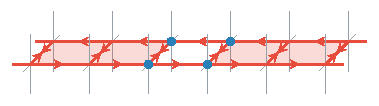
\includegraphics{Figs/lambdarenorm.pdf}
    \vspace*{-.5em}

  \begin{columns}
  \column{.35\textwidth}
  \begin{itemize}
    \item \color{LightUIBase} Rescales $\lambda$ 
  \end{itemize}
  \column{.35\textwidth}
  \begin{itemize}
    \item \color{LightUIBase} $\lambda \to \lambda(\kappa)$
  \end{itemize}
  \end{columns}
  \end{block}
  

  \begin{block}{Correction to $h_2$}
  \centering
  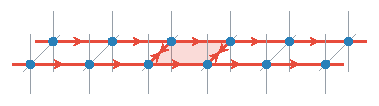
\includegraphics{Figs/h2renorm.pdf}
  \vspace*{-.5em}

  \begin{columns}
  \column{.35\textwidth}
  \begin{itemize}
    \item \color{LightUIBase} Rescales $h_2$ 
  \end{itemize}
  \column{.35\textwidth}
  \begin{itemize}
    \item \color{LightUIBase} $h_2 \to h_2(\beta)$
  \end{itemize}
  \end{columns}
  \end{block}

  \note
  {
    One can of course mix the terms from the two different expansions we are carrying out. Two examples of the possible terms can
    be seen in the figures. For these two simple cases, the mixing will only contribute as a shift in the nearest neighbour
    couplings, and can thus be absorbed by those.

    \vspace{1em}

    There are higher order mixed terms that create entierly new interactions, but those are of much higher order of what we have
    shown here.

    \vspace{1em}

    I will probably skip this slide.
  }

\end{frame}

\begin{frame}
  \frametitle{EoS in lattice units}
  {\centering%
    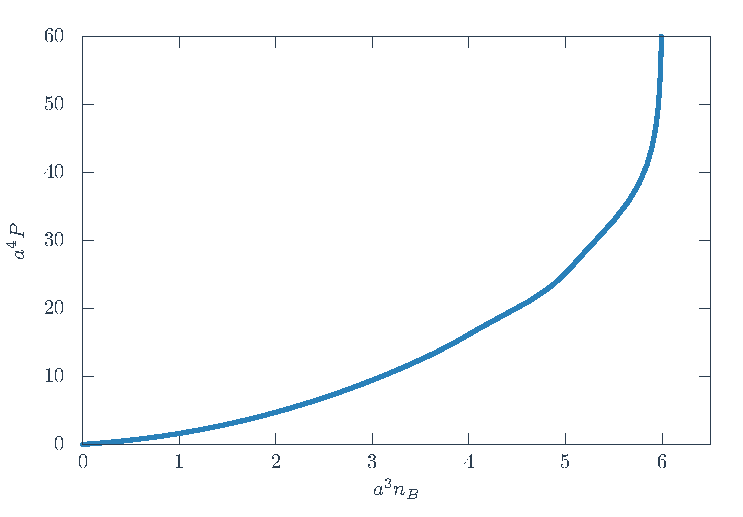
\includegraphics[width=\textwidth]{Figs/eos_lattice_units.pdf}
  \par}
\end{frame}


\end{document}
